\documentclass[a4paper]{article}
\usepackage[top=1in, bottom=1.25in, left=1.25in, right=1.25in]{geometry}
\usepackage{amsmath}
\usepackage{multicol}
\usepackage{graphicx}
\usepackage[utf8]{inputenc}
\usepackage[english]{babel}
\setlength{\parskip}{0.03cm plus4mm minus3mm}
\RequirePackage{ltxcmds}[2010/12/07]
\usepackage{array}
\usepackage{hyperref}
\renewcommand{\arraystretch}{1.5}
%\setlength{\arrayrulewidth}{1mm}
%opening
\title{Homodyne receiver}

\begin{document}

\maketitle

\clearpage

\section{Homodyne receiver}

This block of code simulates the reception and demodulation of an optical signal (which is the input signal of the system) outputing a binary signal. A simplified schematic representation of this block is shown in figure \ref{MQAM_receiver_block_diagram_simple}.

\begin{figure}[h]
	\centering
	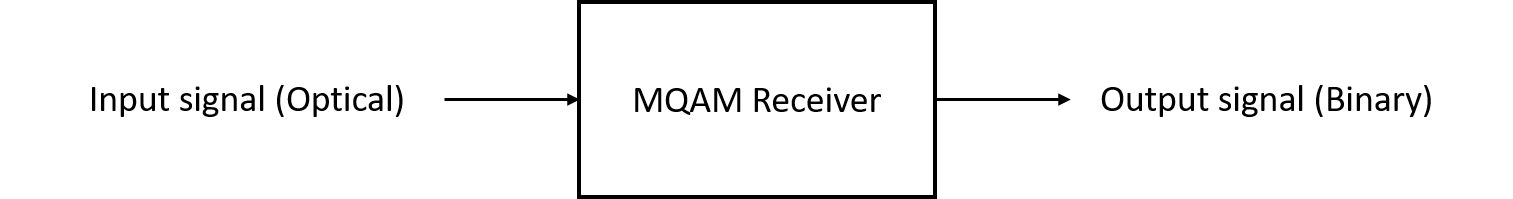
\includegraphics[width=0.8\textwidth]{figures/MQAM_receiver_block_diagram_simple}
	\caption{Basic configuration of the MQAM receiver}\label{MQAM_receiver_block_diagram_simple}
\end{figure}

\subsection*{Functional description}

This block accepts one optical input signal and outputs one binary signal that corresponds to the M-QAM demodulation of the input signal. It is a complex block (as it can be seen from figure \ref{MQAM_receiver_block_diagram}) of code made up of several simpler blocks whose description can be found in the \textit{lib} repository.

In can also be seen from figure \ref{MQAM_receiver_block_diagram} that there's an extra internal (generated inside the homodyne receiver block) input signal generated by the \textit{Clock}. This block is used to provide the sampling frequency to the \textit{Sampler}.


\begin{figure}[h]
	\centering
	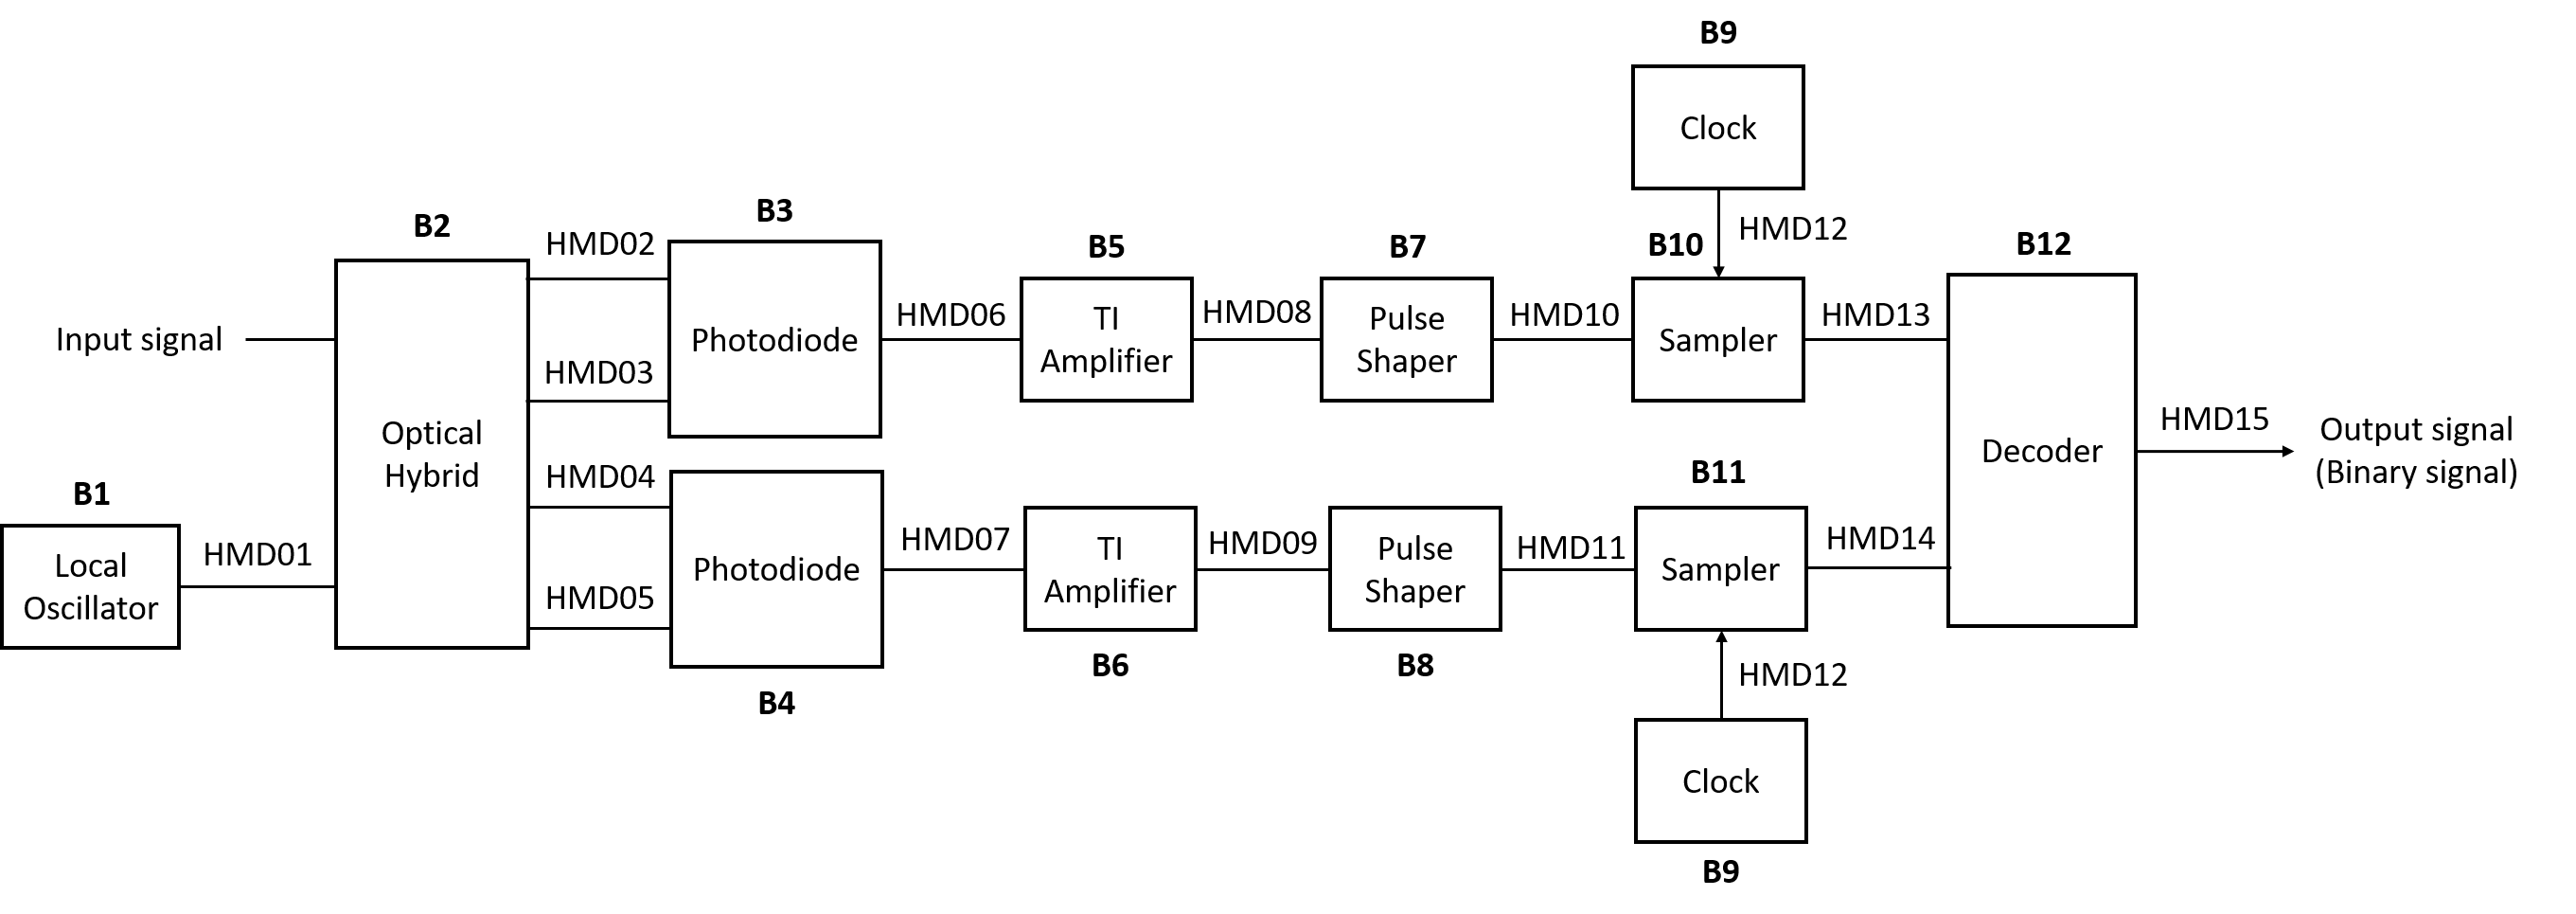
\includegraphics[width=\textwidth]{figures/MQAM_receiver_block_diagram}
	\caption{Schematic representation of the block homodyne receiver.}\label{MQAM_receiver_block_diagram}
\end{figure}

\subsection*{Input parameters}

This block has some input parameters that can be manipulated by the user in order oto change the basic configuration of the receiver. Each parameter has associated a function that allows for its change. In the following table (table~\ref{table}) the input parameters and corresponding functions are summarized.

\begin{table}[h]
	\begin{center}
		\begin{tabular}{| m{3,5cm} | m{5,8cm} |  m{2,5cm} | m{4cm} | }
			\hline
			\textbf{Input parameters} & \textbf{Function} & Type & \textbf{Accepted values} \\ \hline
			IQ amplitudes & setIqAmplitudes & Vector of coordinate points in the I-Q plane & \textbf{Example} for a 4-qam mapping: \{ \{ 1.0, 1.0 \}, \{ -1.0, 1.0 \}, \{ -1.0, -1.0 \}, \{ 1.0, -1.0 \} \} \\ \hline
			Local oscillator power (in dBm) & setLocalOscillatorOpticalPower\_dBm & double(t\_real) & Any double greater than zero\\ \hline
			Local oscillator phase & setLocalOscillatorPhase & double(t\_real) & Any double greater than zero\\ \hline
			Responsivity of the photodiodes & setResponsivity & double(t\_real) &$\in$ [0,1] \\ \hline
			Amplification (of the TI amplifier) & setAmplification & double(t\_real) & Positive real number\\ \hline
			Noise amplitude (introduced by the TI amplifier) & setNoiseAmplitude & double(t\_real) & Real number greater than zero \\ \hline
			Samples to skipe & setSamplesToSkip & int(t\_integer) &  \\ \hline
			Save internal signals & setSaveInternalSignals & bool & True or False\\ \hline
			Sampling period & setSamplingPeriod & double & Givem by \textit{symbolPeriod}/\textit{samplesPerSymbol}\\
			\hline
		\end{tabular}
		\caption{List of input parameters of the block MQAM receiver} \label{table}
	\end{center}
\end{table}

\pagebreak

\subsection*{Methods}

HomodyneReceiver(vector$<$Signal *$>$ \&inputSignal, vector$<$Signal *$>$ \&outputSignal) (\textbf{constructor})
\bigbreak
void setIqAmplitudes(vector$<$t\_iqValues$>$ iqAmplitudesValues)
\bigbreak
vector$<$t\_iqValues$>$ const getIqAmplitudes(void)
\bigbreak
void setLocalOscillatorSamplingPeriod(double sPeriod)
\bigbreak
void setLocalOscillatorOpticalPower(double opticalPower)
\bigbreak
void setLocalOscillatorOpticalPower\_dBm(double opticalPower\_dBm)
\bigbreak
void setLocalOscillatorPhase(double lOscillatorPhase)
\bigbreak
void setLocalOscillatorOpticalWavelength(double lOscillatorWavelength)
\bigbreak
void setSamplingPeriod(double sPeriod)
\bigbreak
void  setResponsivity(t\_real Responsivity)
\bigbreak
void setAmplification(t\_real Amplification)
\bigbreak
void setNoiseAmplitude(t\_real NoiseAmplitude)
\bigbreak
void setImpulseResponseTimeLength(int impResponseTimeLength)
\bigbreak
void setFilterType(PulseShaperFilter fType)
\bigbreak
void setRollOffFactor(double rOffFactor)
\bigbreak
void setClockPeriod(double per)
\bigbreak
void setSamplesToSkip(int sToSkip)

\pagebreak

\subsection*{Input Signals}

\subparagraph*{Number:} 1

\subparagraph*{Type:} Optical signal

\subsection*{Output Signals}

\subparagraph*{Number:} 1

\subparagraph*{Type:} Binary signal

\subsection*{Example}

\subsection*{Sugestions for future improvement}

\clearpage

\section{Local Oscillator}

\begin{tcolorbox}	
	\begin{tabular}{p{2.75cm} p{0.2cm} p{10.5cm}} 	
		\textbf{Header File}   &:& local\_oscillator.h \\
		\textbf{Source File}   &:& local\_oscillator.cpp \\
        \textbf{Version}       &:& 20180130\\
        \textbf{Version}       &:& 20180828 (Romil Patel)\\
	\end{tabular}
\end{tcolorbox}
\subsection*{Version 20180130}
This block simulates a local oscillator with constant power and initial phase. It produces one output complex signal and it doesn't accept input signals.

\subsection*{Input Parameters}

\begin{table}[h]
	\centering
	\begin{tabular}{|c|c|c|c|cccc}
		\cline{1-4}
		\textbf{Parameter} & \textbf{Type} & \textbf{Values} &   \textbf{Default}& \\ \cline{1-4}
		opticalPower & double & any & $1\text{e}-3$ \\ \cline{1-4}
		outputOpticalWavelength & double & any & $1550\text{e}-9$ \\ \cline{1-4}
		outputOpticalFrequency & double & any &  SPEED\_OF\_LIGHT / outputOpticalWavelength \\ \cline{1-4}
		phase & double & $\in \left[0,\frac{\pi}{2}\right]$ & $0$ \\ \cline{1-4}
		samplingPeriod & double & any & $0.0$ \\ \cline{1-4}
        symbolPeriod   & double & any & $0.0$ \\ \cline{1-4}
        signaltoNoiseRatio & double & any & $0.0$ \\ \cline{1-4}
        laserLineWidth & double & any & $0.0$ \\ \cline{1-4}
        laserRIN       & double & any & $0.0$ \\ \cline{1-4}
	\end{tabular}
	\caption{Binary source input parameters}
	\label{table:LO_in_par}
\end{table}

%
%\begin{itemize}
%	\item opticalPower\{ 1e-3 \}
%	\item wavelength\{ 1550e-9 \}
%	\item frequency\{ SPEED\_OF\_LIGHT / wavelength \}
%	\item phase\{ 0 \}
%	\item samplingPeriod\{ 0.0 \}
%\end{itemize}

\subsection*{Methods}

LocalOscillator() {}
\bigbreak
LocalOscillator(vector$<$Signal *$>$ \&InputSig, vector$<$Signal *$>$ \&OutputSig) :Block(InputSig, OutputSig)\{\};
\bigbreak
void initialize(void);
\bigbreak
bool runBlock(void);
\bigbreak
void setSamplingPeriod(double sPeriod);
\bigbreak
void setSymbolPeriod(double sPeriod);
\bigbreak
void setOpticalPower(double oPower);
\bigbreak
void setOpticalPower\_dBm(double oPower\_dBm);
\bigbreak
void setWavelength(double wlength);
\bigbreak
void setFrequency(double freq);
\bigbreak
void setPhase(double lOscillatorPhase);
\bigbreak
void setSignaltoNoiseRatio(double sNoiseRatio);
\bigbreak
void setLaserLinewidth(double laserLinewidth);
\bigbreak
void setLaserRIN(double laserRIN);

\subsection*{Functional description}

This block generates a complex signal with a specified phase given by the input parameter \textit{phase}.

\subsection*{Input Signals}

\textbf{Number:} 0

\subsection*{Output Signals}

\textbf{Number:} 1\\
\textbf{Type:} Optical signal

\subsection*{Version 20180828}


\clearpage

\section{Optical Hybrid}

\begin{tcolorbox}	
	\begin{tabular}{p{2.75cm} p{0.2cm} p{10.5cm}} 	
		\textbf{Header File}   &:& optical\_hybrid.h \\
		\textbf{Source File}   &:& optical\_hybrid.cpp \\
	\end{tabular}
\end{tcolorbox}

This block simulates an optical hybrid. It accepts two input signals corresponding to the signal and to the local oscillator. It generates four output complex signals separated by $90^\circ$ in the complex plane. Figure ~\ref{opticalhybrid} shows a schematic representation of this block.

\begin{figure}[h]
	\centering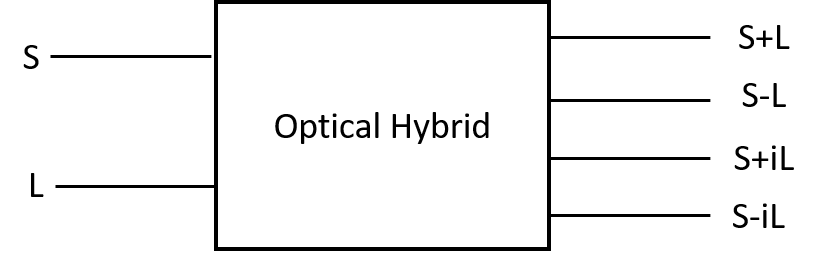
\includegraphics[width=0.6\textwidth]{./lib/optical_hybrid/figures/optical_hybrid_block_diagram.png}
	\caption{Schematic representation of an optical hybrid.}\label{opticalhybrid}
\end{figure}

\subsection*{Input Parameters}

\begin{table}[h]
	\centering
	\begin{tabular}{|c|c|c|c|ccp{60mm}}
		\cline{1-4}
		\textbf{Parameter} & \textbf{Type} & \textbf{Values} &   \textbf{Default}& \\ \cline{1-4}
		outputOpticalPower & double & any & $1e-3$ \\ \cline{1-4}
		outputOpticalWavelength & double & any & $1550e-9$ \\ \cline{1-4}
		outputOpticalFrequency & double & any & SPEED\_OF\_LIGHT / outputOpticalWavelength \\ \cline{1-4}
		powerFactor & double & $\leq 1$ & $0.5$ \\ \cline{1-4} 
	\end{tabular}
	\caption{Optical hybrid input parameters}
	\label{table:optical_hybrid_in_par}
\end{table}

%\begin{itemize}
%	\item outputOpticalPower\{ 1e-3 \} 
%	\item outputOpticalWavelength\{ 1550e-9 \}
%	\item outputOpticalFrequency\{ SPEED\_OF\_LIGHT / wavelength \}
%	\item powerFactor\{0.5\}
%\end{itemize}

\subsection*{Methods}
 
OpticalHybrid() {}
\bigbreak
OpticalHybrid(vector$<$Signal *$>$ \&InputSig, vector$<$Signal *$>$ \&OutputSig) :Block(InputSig, OutputSig) {}
\bigbreak
void initialize(void)
\bigbreak
bool runBlock(void)
\bigbreak
void setOutputOpticalPower(double outOpticalPower)
\bigbreak
void setOutputOpticalPower\_dBm(double outOpticalPower\_dBm)
\bigbreak
void setOutputOpticalWavelength(double outOpticalWavelength)
\bigbreak
void setOutputOpticalFrequency(double outOpticalFrequency) 
\bigbreak
void setPowerFactor(double pFactor)

\subsection*{Functional description}

This block accepts two  input signals corresponding to the signal to be demodulated ($S$) and to the local oscillator ($L$). It generates four output optical signals given by $\textit{powerFactor}\times(S+L)$, $\textit{powerFactor}\times(S-L)$,$\textit{powerFactor}\times(S+iL)$, $\textit{powerFactor}\times(S-iL)$. The input parameter \textit{powerFactor} assures the conservation of optical power.

\subsection*{Input Signals}

\subparagraph*{Number:} 2

\subparagraph*{Type:} Optical (OpticalSignal)

\subsection*{Output Signals}

\subparagraph*{Number:} 4

\subparagraph*{Type:} Optical (OpticalSignal)

\subsection*{Examples} 

%\begin{figure}[h]
%	\centering
%	\includegraphics[width=\textwidth]{./lib/optical_hybrid/MQAM_optical_hybrid_output.pdf}
%	\caption{Example of one of the output signals of this block for a binary sequence 01}\label{OpticalHybrid_output}
%\end{figure}

\subsection*{Sugestions for future improvement}

\clearpage

\section{Photodiode pair}

\begin{tcolorbox}	
	\begin{tabular}{p{2.75cm} p{0.2cm} p{10.5cm}} 	
		\textbf{Header File}   &:& photodiode\_old.h \\
		\textbf{Source File}   &:& photodiode\_old.cpp \\
	\end{tabular}
\end{tcolorbox}


This block simulates a block of two photodiodes assembled like in figure~\ref{photodiode}. It accepts two optical input signals and outputs one electrical signal. Each photodiode converts an optical signal to an electrical signal. The two electrical signals are then subtracted and the resulting signals corresponds to the output signal of the block.

\begin{figure}[h]
	\centering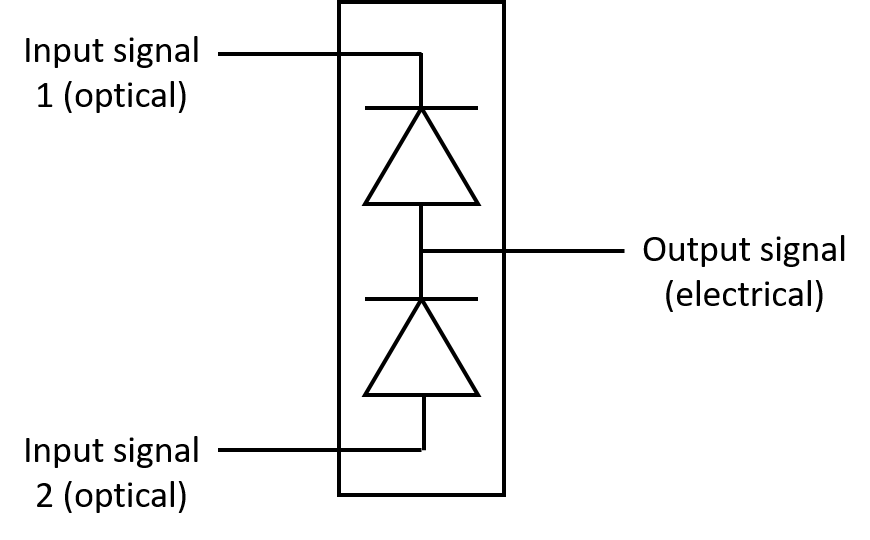
\includegraphics[width=0.5\textwidth]{./lib/photodiode/figures/photodiode.png}
	\caption{Schematic representation of the physical equivalent of the photodiode code block.}\label{photodiode}
\end{figure}

\subsection*{Input Parameters}

\begin{itemize}
	\item responsivity\{1\}
	\item outputOpticalWavelength\{ 1550e-9 \}
	\item outputOpticalFrequency\{ SPEED\_OF\_LIGHT / wavelength \}
\end{itemize}

\subsection*{Methods}
 
Photodiode() {}
\bigbreak
Photodiode(vector$<$Signal *$>$ \&InputSig, vector$<$Signal *$>$ \&OutputSig) :Block(InputSig, OutputSig) {}
\bigbreak
void initialize(void)
\bigbreak
bool runBlock(void)
\bigbreak
void setResponsivity(\texttt{t\_real} Responsivity)

\subsection*{Functional description}

This block accepts two input optical signals. It computes the optical power of the signal (given by the absolute value squared of the input signal) and multiplies it by the \textit{responsivity} of the photodiode. This product corresponds to the current generated by the photodiode. This is done for each of the input signals. The two currents are then subtracted producing a single output current, that corresponds to the output electrical signal of the block.

\subsection*{Input Signals}

\subparagraph*{Number:} 2

\subparagraph*{Type:} Optical (OpticalSignal)

\subsection*{Output Signals}

\subparagraph*{Number:} 1

\subparagraph*{Type:} Electrical (TimeContinuousAmplitudeContinuousReal)

\subsection*{Examples} 

\begin{figure}[h]
	\centering
	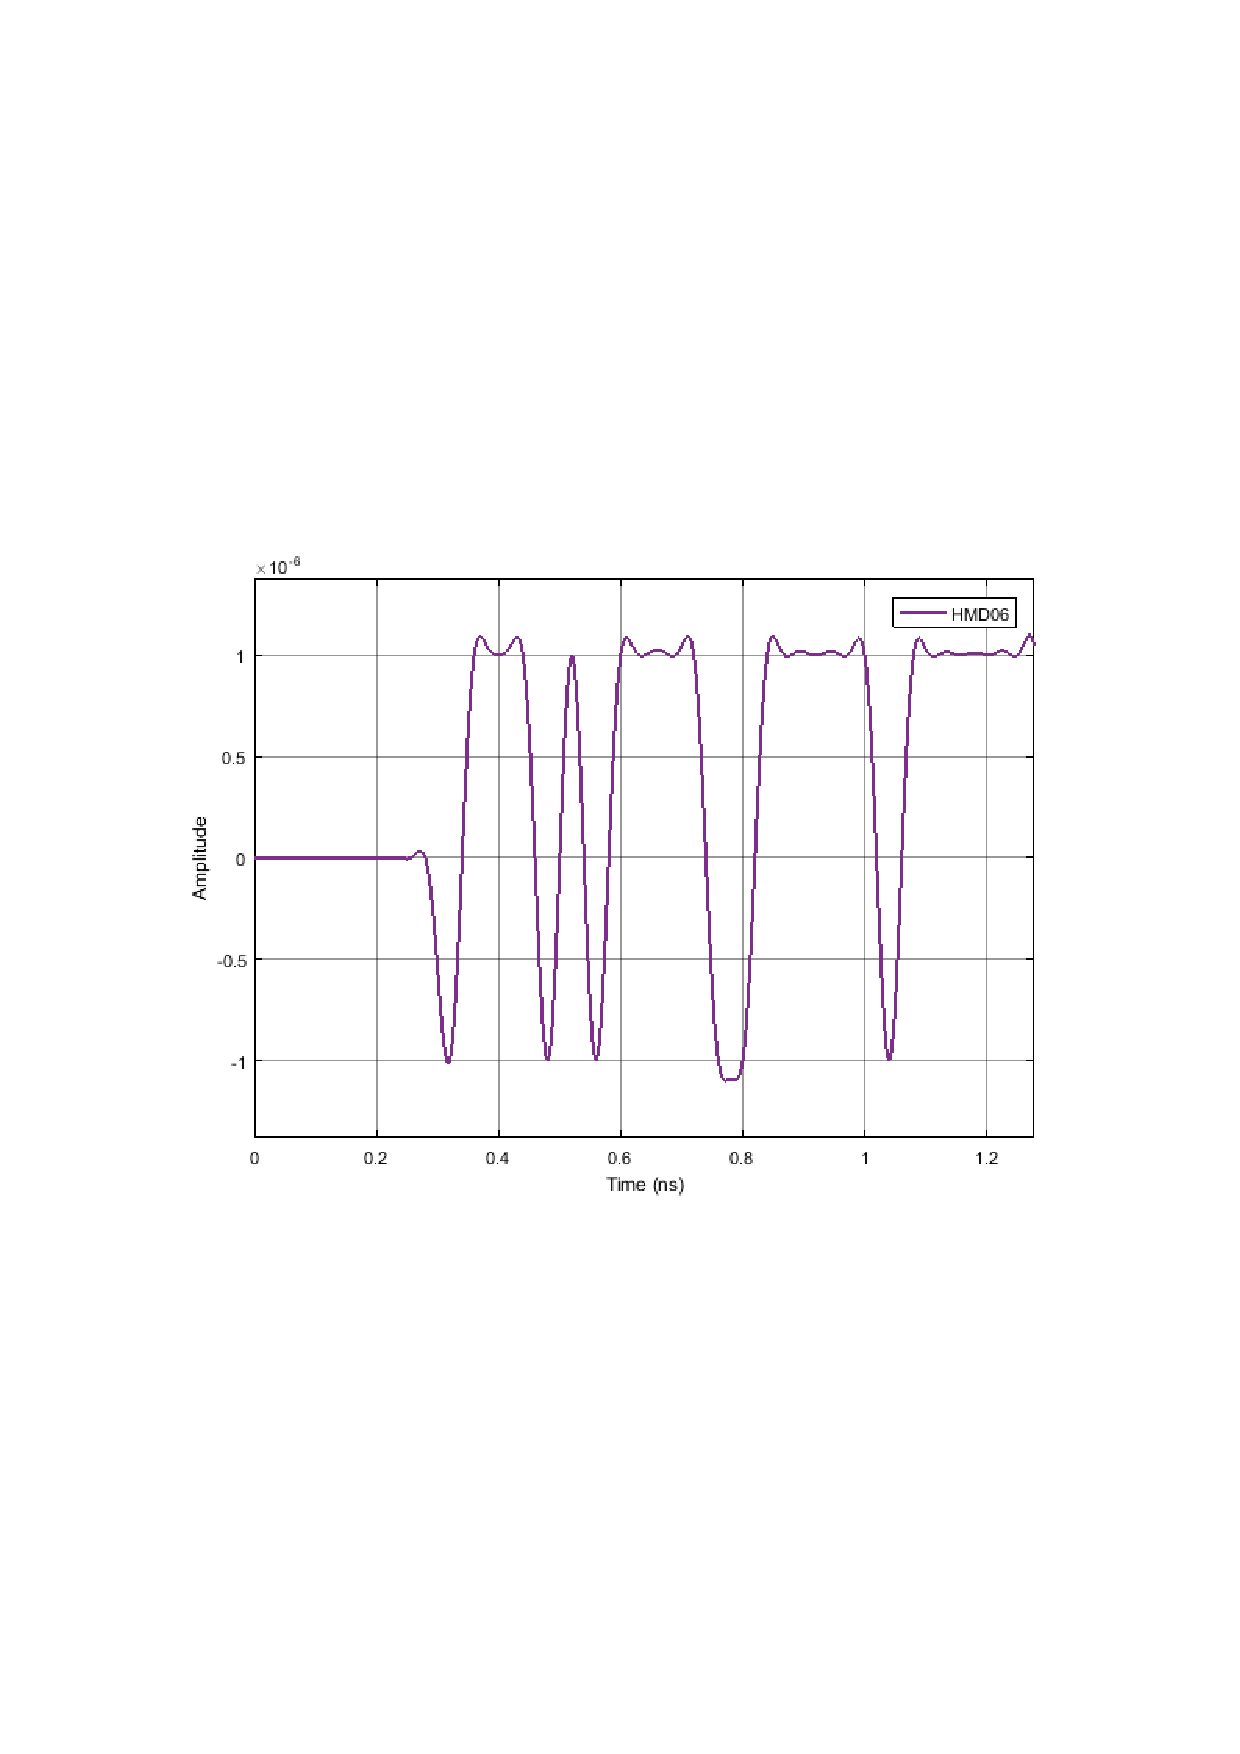
\includegraphics[clip, trim=0.5cm 9cm 0.5cm 9cm, width=\textwidth]{./lib/photodiode/figures/MQAM_photodiode_old_output.pdf}
	\caption{Example of the output singal of the photodiode block for a bunary sequence 01}\label{Photodiode_output}
\end{figure}

\subsection*{Sugestions for future improvement}


\clearpage

\section{TI Amplifier}

\maketitle

This block has one input signal and one output signal both corresponding to electrical signals. The output signal corresponds to the amplification of the input signal with added noise.


\subsection*{Input Parameters}

\begin{itemize}
	\item amplification\{1e6\}
	\item noiseamp\{ 1e-4 \}
\end{itemize}

\subsection*{Methods}
 
TIAmplifier() {}
\bigbreak
TIAmplifier(vector$<$Signal *$>$ \&InputSig, vector$<$Signal *$>$ \&OutputSig) :Block(InputSig, OutputSig) {}
\bigbreak
void initialize(void)
\bigbreak
bool runBlock(void)
\bigbreak
void setAmpplification(\texttt{t\_real} Amplification)
\bigbreak
void setNoiseAmpplitude(\texttt{t\_real} NoiseAmplitude)

\subsection*{Functional description}

The output signal is the product of the input signal with the parameter \textit{amplification} plus a component that corresponds to the noise introduced by the amplification of the signal. 

\pagebreak

\subsection*{Input Signals}

\subparagraph*{Number:} 1

\subparagraph*{Type:} Electrical (TimeContinuousAmplitudeContinuousReal)

\subsection*{Output Signals}

\subparagraph*{Number:} 1

\subparagraph*{Type:} Electrical (TimeContinuousAmplitudeContinuousReal)

\subsection*{Examples} 

\begin{figure}[h]
	\centering
	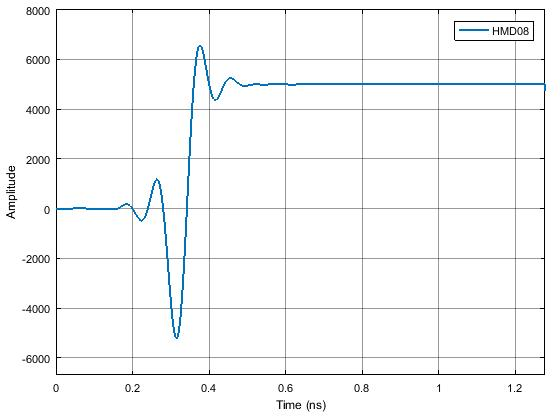
\includegraphics[width=\textwidth]{../homodyne_receiver/figures/TIAmplifier_output}
	\caption{Example of the output signal of the amplifier block for a binary sequence 01. Note the scale of the y axis in comparison to the one in the output signal of the photodiode. The shape of the signal is the same as expected}\label{TIAmplifier_output}
\end{figure}

\subsection*{Sugestions for future improvement}


\documentclass[../../sdf/tex/BPSK_system.tex]{subfiles}
\graphicspath{{../../images/}}
%opening
\onlyinsubfile{\title{Pulse Shaper}}
\date{}


\begin{document}

\maketitle

This blocks applies a time domain, finite impulse response filter to the signal. The filter's transfer function is defined by the vector \textit{impulseResponse}. It allows for passive filter mode operation via a boolean check.

\subsection*{Input Parameters}

\begin{itemize}
	\item filterType
	\item impulseResponseTimeLength
	\item rollOfFactor
	\item usePassiveFilterMode
\end{itemize}

\subsection*{Functional Description}

\subsection*{Input Signals}

\textbf{Number}: 1

\textbf{Type}: Sequence of Dirac Delta functions (ContinuousTimeDiscreteAmplitude)

\subsection*{Output Signals}

\textbf{Number}: 1

\textbf{Type}: Sequence of impulses modulated by the filter (ContinuousTimeContiousAmplitude)

\subsection*{Suggestions for future improvement}

Introduce other types of filters.

\end{document}
\documentclass[../../sdf/tex/BPSK_system.tex]{subfiles}
\graphicspath{{../../images/}}
%opening
\onlyinsubfile{\title{Sampler}}
\date{ }

\begin{document}

\onlyinsubfile{\maketitle}

\subsection*{Input Parameters}

\begin{multicols}{2}
	\begin{itemize}
		\item setSamplingRate
		\item setDelay
	\end{itemize}
\end{multicols}

\subsection*{Functional Description}

This block accepts one real continuous signal and outputs one real discrete signal built from a sampling of the input signal with a predetermined sampling rate. The sampling rate is defined by the value \textit{SamplingRate}. This block also allows for a controlled adjustment of the starting point of the output signal, defined by the value \textit{Delay}

\subsection*{Input Signals}

\textbf{Number}: 1

\textbf{Type}: Real signal (ContinuousTimeContinuousAmplitude)

\subsection*{Output Signals}

\textbf{Number}: 1

\textbf{Type}: Real signal (DiscreteTimeContinuousAmplitude)

\end{document}
\clearpage

\section{Clock}

\begin{tcolorbox}	
	\begin{tabular}{p{2.75cm} p{0.2cm} p{10.5cm}} 	
		\textbf{Header File}   &:& clock.h \\
		\textbf{Source File}   &:& clock.cpp \\
	\end{tabular}
\end{tcolorbox}

This block doesn't accept any input signal. It outputs one signal that corresponds to a sequence of Dirac's delta functions with a user defined \textit{period}.

\subsection*{Input Parameters}

%\begin{itemize}
%	\item period\{ 0.0 \};
%	\item samplingPeriod\{ 0.0 \};
%\end{itemize}

\begin{table}[h]
	\centering
	\begin{tabular}{|c|c|c|c|cccc}
		\cline{1-4}
		\textbf{Parameter} & \textbf{Type} & \textbf{Values} &   \textbf{Default}& \\ \cline{1-4}
		period & double & any & $0.0$ \\ \cline{1-4}
		samplingPeriod & double & any & $0.0$ \\ \cline{1-4}
	\end{tabular}
	\caption{Binary source input parameters}
	\label{table:clock_in_par}
\end{table}

\subsection*{Methods}

Clock() {}
\bigbreak
Clock(vector$<$Signal *$>$ \&InputSig, vector$<$Signal *$>$ \&OutputSig) :Block(InputSig, OutputSig) {}
\bigbreak
void initialize(void)
\bigbreak
bool runBlock(void)
\bigbreak
void setClockPeriod(double per)
\bigbreak
void setSamplingPeriod(double sPeriod)

\subsection*{Functional description}


\pagebreak

\subsection*{Input Signals}

\subparagraph*{Number:} 0

\subsection*{Output Signals}

\subparagraph*{Number:} 1

\subparagraph*{Type:} Sequence of Dirac's delta functions. (TimeContinuousAmplitudeContinuousReal)

\subsection*{Examples}

%\begin{figure}[h]
%	\centering
%	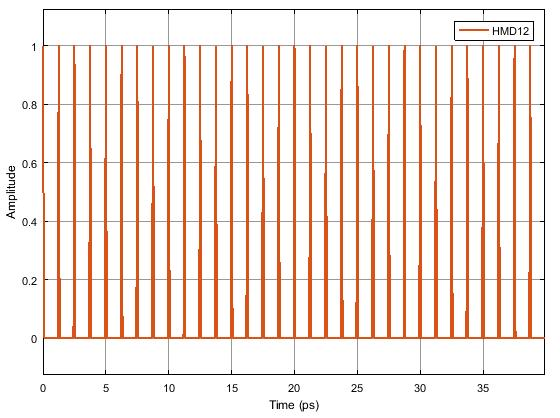
\includegraphics[width=\textwidth]{./lib/clock/figures/Clock_output}
%	\caption{Example of the output signal of the clock}\label{Clock_output}
%\end{figure}

\subsection*{Sugestions for future improvement}


\clearpage

\section{Decoder}

This block accepts a complex electrical signal and outputs a sequence of binary values (0's and 1's). Each point of the input signal corresponds to a pair of bits.

\subsection*{Input Parameters}

\begin{itemize}
	\item\texttt{t\_integer} m\{ 4 \}
	\item vector$<$\texttt{t\_complex}$>$ iqAmplitudes\{ \{ 1.0, 1.0 \},\{ -1.0, 1.0 \},\{ -1.0, -1.0 \},\{ 1.0, -1.0 \} \};
\end{itemize}

\subsection*{Methods}
 
Decoder() {}
\bigbreak
Decoder(vector$<$Signal *$>$ \&InputSig, vector$<$Signal *$>$ \&OutputSig) :Block(InputSig, OutputSig) {}
\bigbreak
void initialize(void)
\bigbreak
bool runBlock(void)
\bigbreak
void setM(int mValue)
\bigbreak
void getM()
\bigbreak
void setIqAmplitudes(vector$<$\texttt{t\_iqValues}$>$ iqAmplitudesValues)
\bigbreak
vector$<$\texttt{t\_iqValues}$>$getIqAmplitudes()

\subsection*{Functional description}

This block makes the correspondence between a complex electrical signal and pair of binary values using a predetermined constellation.

To do so it computes the distance in the complex plane between each value of the input signal and each value of the \textit{iqAmplitudes} vector selecting only the shortest one. It then converts the point in the IQ plane to a pair of bits making the correspondence between the input signal and a pair of bits.

\pagebreak

\subsection*{Input Signals}

\subparagraph*{Number:} 1

\subparagraph*{Type:} Electrical complex (TimeContinuousAmplitudeContinuousReal)

\subsection*{Output Signals}

\subparagraph*{Number:} 1

\subparagraph*{Type:} Binary 

\subsection*{Examples}

As an example take an input signal with positive real and imaginary parts. It would correspond to the first point of the \textit{iqAmplitudes} vector and therefore it would be associated to the  pair of bits $00$. 

\begin{figure}[h]
	\centering
	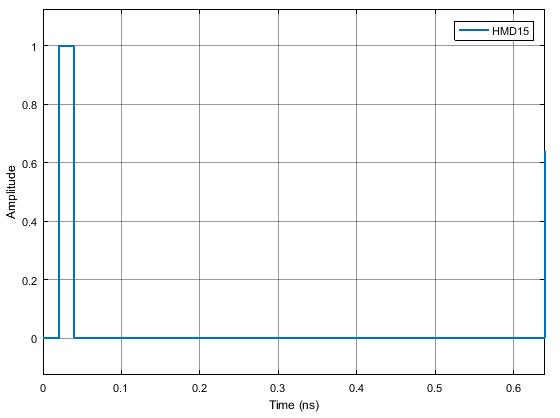
\includegraphics[width=\textwidth]{../homodyne_receiver/figures/Decoder_output}
	\caption{Example of the output signal of the decoder for a binary sequence 01. As expected it reproduces the initial bit stream}\label{Decoder_output}
\end{figure}

\subsection*{Sugestions for future improvement}


\end{document} 